\documentclass [11pt]{report}
\usepackage{graphicx}
\usepackage{amssymb,amsmath}
%\usepackage[sorting=none]{biblatex}
\bibliographystyle{unsrt}
\usepackage{url}
\usepackage{listings}
\usepackage[a4paper,bindingoffset=0.2in,left=0.8in,right=0.8in,top=0.8in,bottom=1in,footskip=.25in]{geometry}
\begin {document}

\title{CS296 Project : Simulation of a Hand gun in Box2D}
\author{
    HAREN SAGA\\
    120050072\\
    120050072@iitb.ac.in
      \and
    NISHANT KUMAR SINGH\\  
    120050043\\
    120050043@iitb.ac.in
    \and
    VARUN TELUGUNTLA\\
    120050077\\
   120050077@iitb.ac.in
}

\date{\today}

\maketitle

\section{Introduction}
~\cite{sahg}.
A semi-automatic pistol is a type of handgun which uses a single chamber and barrel, with a mechanism powered by the previous shot to load a fresh cartridge into the chamber. One round is fired each time the trigger of a semi-automatic pistol is pulled.A semi-automatic pistol harnesses the energy of one shot to reload the chamber for the next, typically via recoil operation, blowback, or gas operation. After a round is fired, the spent casing is ejected and a new round from the magazine is loaded into the chamber, allowing another shot to be fired as soon as the trigger is again pulled. 


\section{Original Design of the gun~\cite{utubesource}.}
\begin{center}
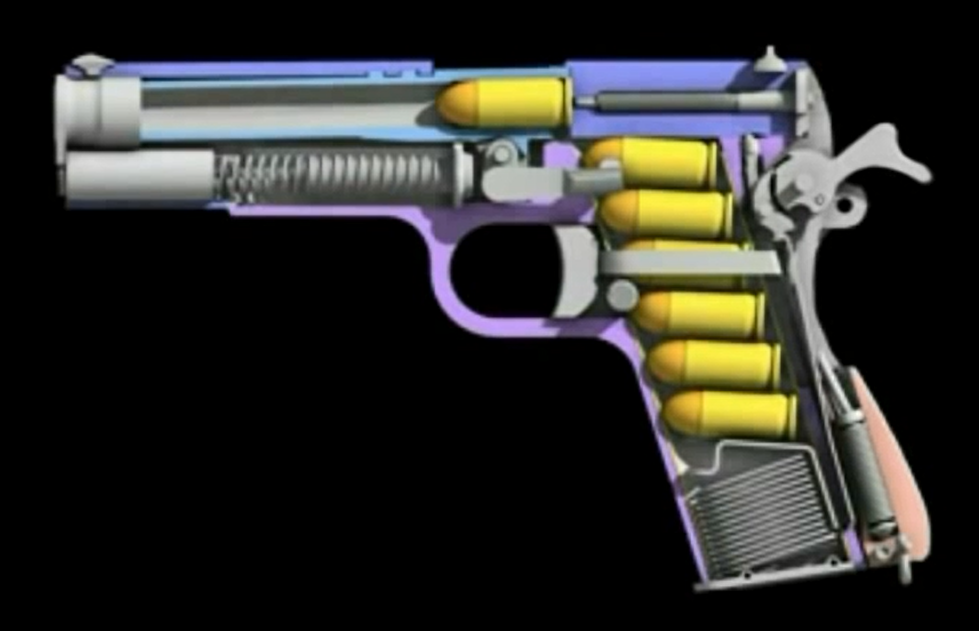
\includegraphics[scale=0.5]{./images/actgun.png}
\end{center}
\section{Original Inkscape Drawing~\cite{ink}.} 

\begin{center}
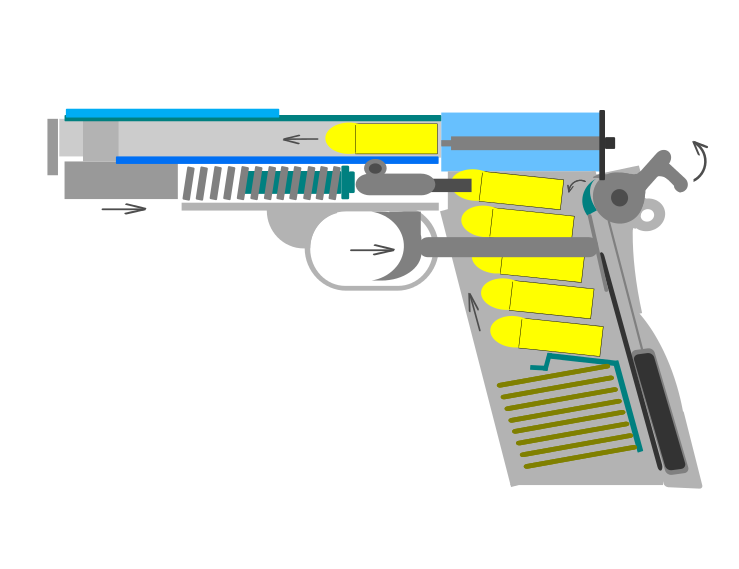
\includegraphics[scale=0.6]{./images/gunink.png}
\end{center}
\section{Finished Design of the gun}
\begin{center}
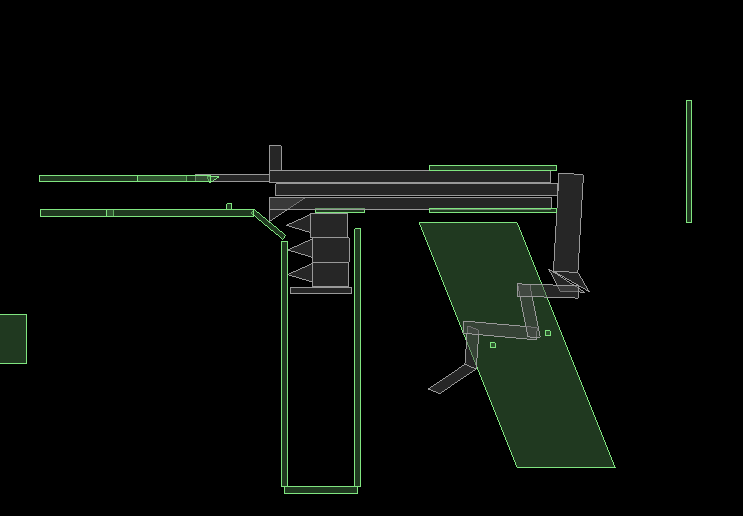
\includegraphics[scale=0.5]{./images/gun.png}
\end{center}
\section{About the finished design}
There is a marked variation in the originally intended design and what was finally made. First let us have a look at the differences:\\ 
\newline
1. In the original design the magazine is incorporated into the handle of the gun. This is an essential feature for the handgun as it makes it compact. In the finished design the bullet-holder i.e. the magazine has been kept separately and in the front of the trigger and the handle. This makes the finished design look more like an assault rifle.
\begin{center}
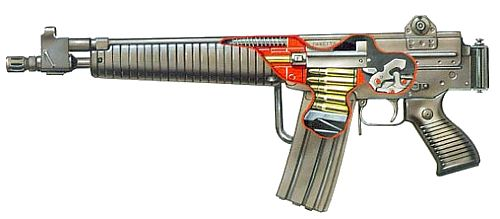
\includegraphics[scale=0.4]{./images/assault.jpg}
\end{center}
2. The trigger mechanism is slightly different as can be seen from the two figures ,the inkscape drawing and the actual simulation.\\
Now, talking about the finished design:
~\cite{b2dm}.
\subsection{Bullets}
Bullet has been designed simply by taking a rectanglular body and a triangular body and attaching them with Revolute joint.
\subsection{Magazine}
Magazine is basically the bullet container. In its design goes three rectangular slabs to enclose the container and one bullet stand on which the bullets lie. Two distance joints ensure that the bullet stand is pushing the bullets upward. A prismatic joint has been put for the stand which cancels its motion along horizontal axis.
\subsection{Trigger Mechanism}
The trigger mechanism has been designed by using polygons and defining multiple fixtures for the same body. Appropriate revolutejoints have been added at places to function as the hinges. The main trigger has been attached to the hammer stopper using a rod which is nothing but a rectangular body. Motor has been used to function as spring to keep the trigger in place tightly.
\subsection{The hammer}
The hammer is nothing but a body with two fixtures one of which has the shape of a rectangle and other which is a triangle. Revolutejoint has been added to function as the hinge of the hammer. Motor has been used to mimic the spring which twists the hammer so as to hit the hitting pin.
\subsection{The pullback mechanism}
This mechanism is responsible for loading the gun. It also contains the hitting pin. The pullback mechanism consists of three bodies two of which in a sense enclose the hitting pin. The hitting pin is a rectangular body. The enclosers are bodies with two fixtures defined on them one of which is a rectangular object and the other triangular object for the lower part and a rectangular object for the upper portion. Distance joints have been used to keep the hitting pin in place. Four such joints have been placed. Two other distance joints have been used which function as the spring which is responsible for bringing the mechanism back after the gun has been loaded.
Also, in the pullback mechanism a rectangular slab has been attached to the top portion which facilitates proper loading of bullets into the barrel.
\subsection{The barrel}
The barrel consists of two rectangular slabs the upper one being slightly smaller in length than the lower one. This is to allow the spent bullet shell to fly out of the gun after it has been fired.



\section{Working}
\subsection{Actual}
~\cite{utubeanim}.
The basic principle of the pistol is recoil operation. As the expanding combustion gases force the bullet down the barrel, they give reverse momentum to the slide and barrel which are locked together during this portion of the firing cycle. After the bullet has left the barrel, the slide and barrel continue rearward a short distance.
At this point, a link pivots the rear of the barrel down, out of locking recesses in the slide, and the barrel is stopped by contact of the lower barrel lugs against the frame's vertical impact surface. As the slide continues rearward, a claw extractor pulls the spent casing from the firing chamber and an ejector strikes the rear of the case, pivoting it out and away from the pistol. The slide stops and is then propelled forward by a spring to strip a fresh cartridge from the magazine and feed it into the firing chamber. At the forward end of its travel, the slide locks into the barrel and is ready to fire again. 
\subsection{Our Design}
The working of our design is very similar to how the original gun works. Conditions have been written in place of actual physics behind the working. \\
 Such as, if the hitting pin collides with bullet's back, the joints between the bullethead and the shell breaks and the head gets an impulse in the forward direction. The shell gets an impulse in the upward direction. The effect of combustion gases has not exactly been simulated rather has been duplicated by the conditional statements.The following code snippet is responsible for firing the bullet i.e. applying impulses:\\ 
 ~\cite{desjoint}.
 \begin{lstlisting}
// The situation when one bullet has been fired i.e. 
//now the gun has to automatically
//  reload
if(reload){
// Check which bullet has been fired and 
//destroy that particular joint.
  for(int j =0 ;j<3;j++){
    if(jointdestroy[j]) {
      jointdestroy[j] = false;
      if(joint_1[j] != NULL){
        m_world->DestroyJoint(joint_1[j]);
        joint_1[j] = NULL;
      }
      if(joint_2[j] != NULL){
        m_world->DestroyJoint(joint_2[j]);
        joint_2[j] = NULL;
      }
// Give linear impulse to bullethead and almost-vertical impulse 
//to the shell
    body_bulhead[j]->ApplyLinearImpulse(b2Vec2(-1000,0),
                      body_bulhead[j]->GetWorldCenter(),true);
    body_bul[j]->ApplyLinearImpulse(b2Vec2(2,1000),
                 body_bul[j]->GetWorldCenter(),true);
			}
	}
	}
\end{lstlisting} 
 
 The hammer gets locked by the stopper as the pullback mechanism (analogous to the slide above) moves back. The pullback mechanism is then propelled forward by the distance joint functioning as the spring. In its way the slide's lower end gets stuck against the bullet and drags it along into the barrel. The gun is now ready to fire another bullet. The following part of the code is responsible for reloading the gun
 ~\cite{force2d}.
\begin{lstlisting}
// The automatic reloading of the gun.
if(reload){
  if(i%2==0 && i<30){
  body_pb->ApplyForce(b2Vec2(5000,0),body_pb->GetWorldCenter(),true);
  body_pb1->ApplyForce(b2Vec2(5000,0),body_pb1->GetWorldCenter(),true);
  }
  i++;
  if(i>100 && automatic){
  reload = false;
  for(int z =0 ;z<30;z++){
    body_t->ApplyForce(b2Vec2(100,0),b2Vec2(body_t->GetWorldCenter().x-1.0f
    ,body_t->GetWorldCenter().y-4.0f),true);
	}
	i = 0;
}
}
\end{lstlisting} 
\section{Working : Explained using images from the simulation}
1. Pulling the slide back loads the gun.\newline
\begin{center}

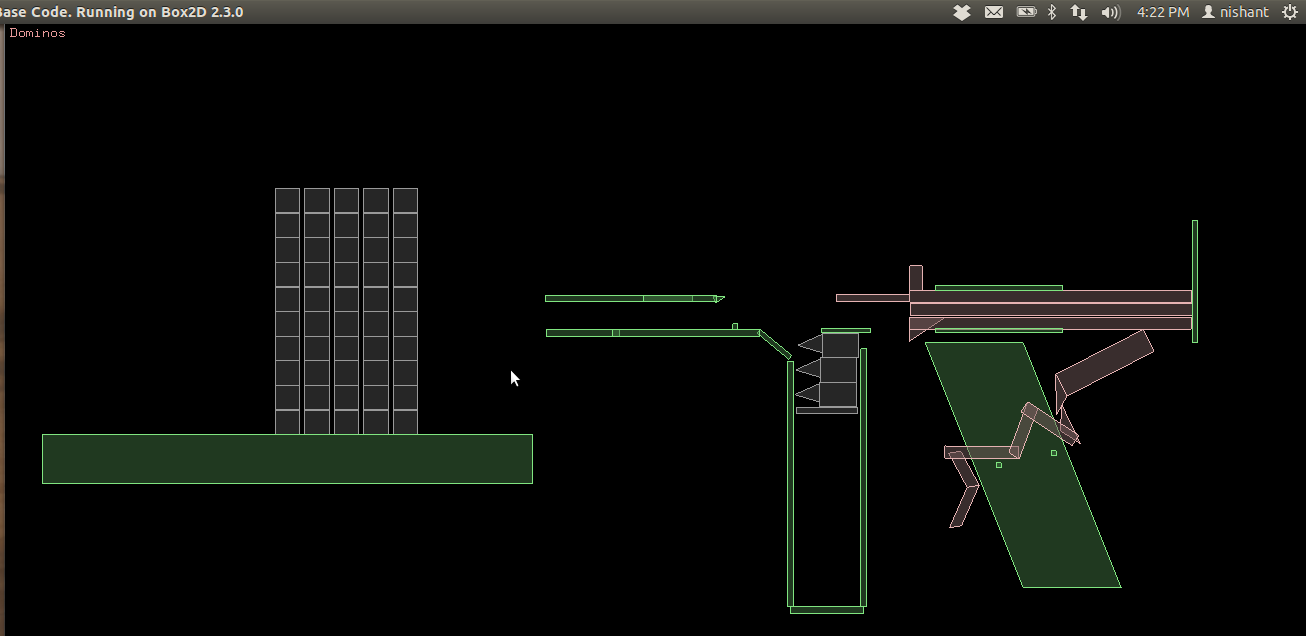
\includegraphics[scale=0.3]{./images/loading.png}\\
\end{center}
2. The bullet begin taken up into the barrel as the slide returns.\newline
\begin{center}
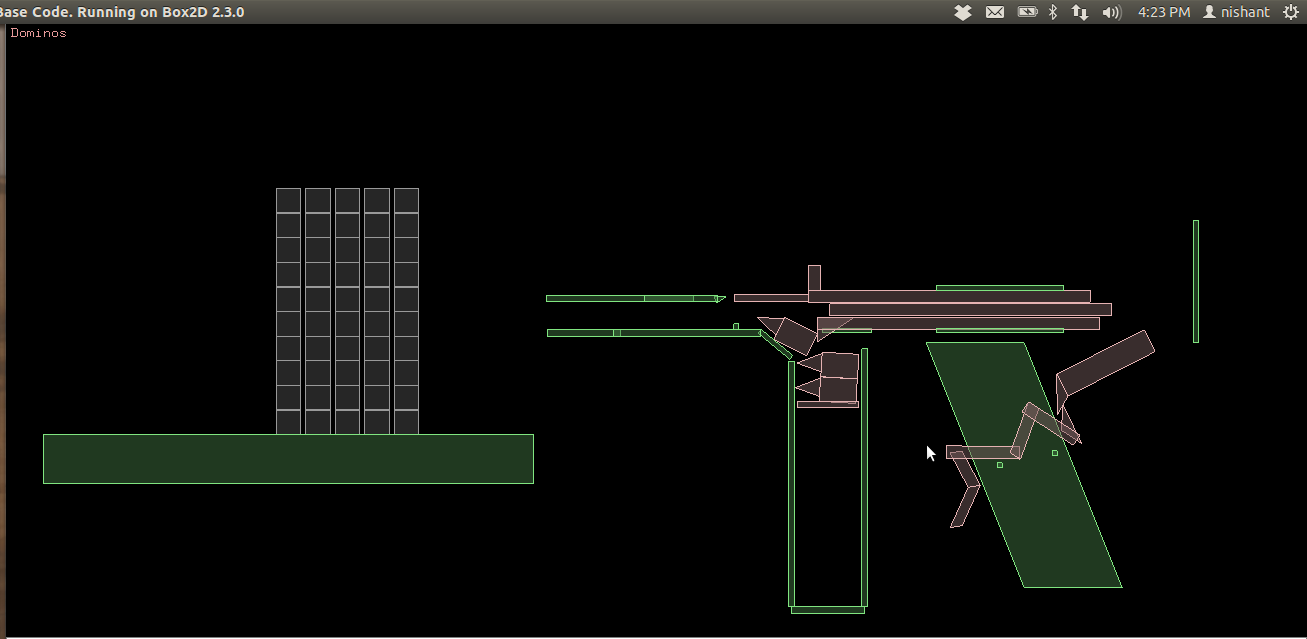
\includegraphics[scale=0.3]{./images/bulletup.png}\\

\end{center}
3. The gun in the loaded state.\newline
\begin{center}
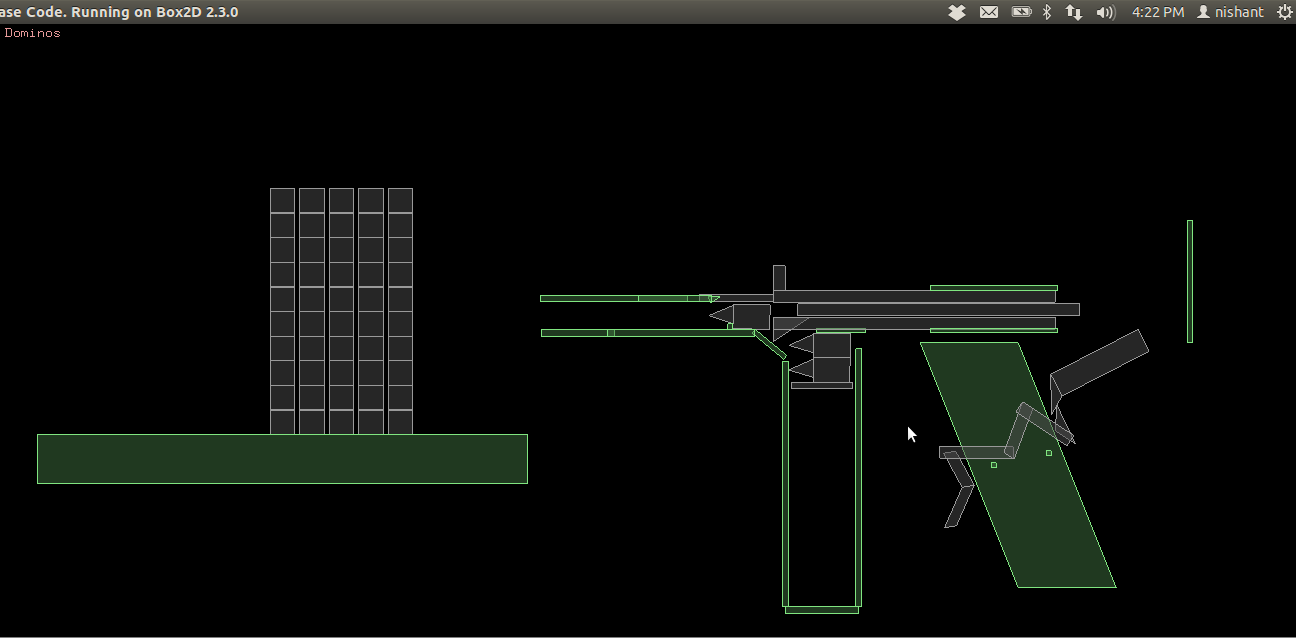
\includegraphics[scale=0.3]{./images/loaded.png}\\
\end{center}
4. One bullet has been fired.\newline
\begin{center}
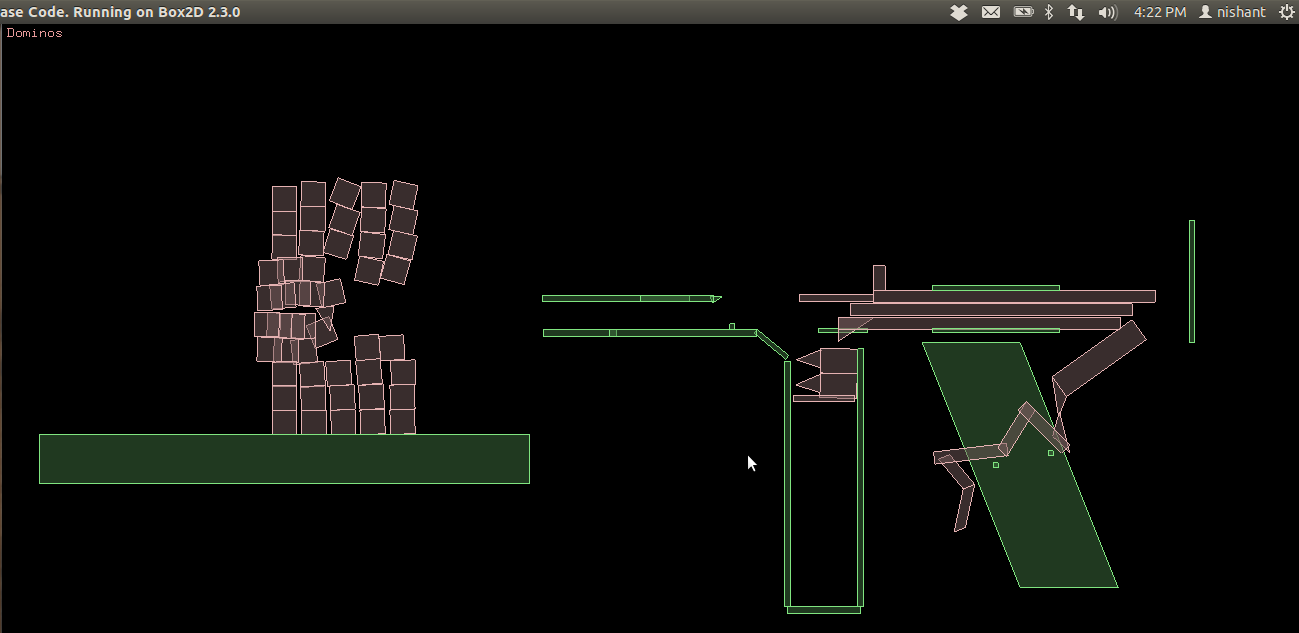
\includegraphics[scale=0.3]{./images/fired.png}\\

\end{center}
\section{Analysing the plots}
~\cite{mplib}.
\subsection{Observations from Plot 01}
Observing the first plot ,we see that the averaged loop time increases with the iteration value, on the contrary, the averaged step time decreases with increasing iteration values. The increase in average loop time can be easily explained as follows. Each iteration will trivially take roughly the same amount of time. Thus increasing number of iterations will linearly increase the loop time. The decrease in averaged step time can be attributed to the fact that towards the end of simulation most of the events have occured and in the beginning, step time will include the time required to set the objects to their respective stable positions so initially it is large.
\begin{center}
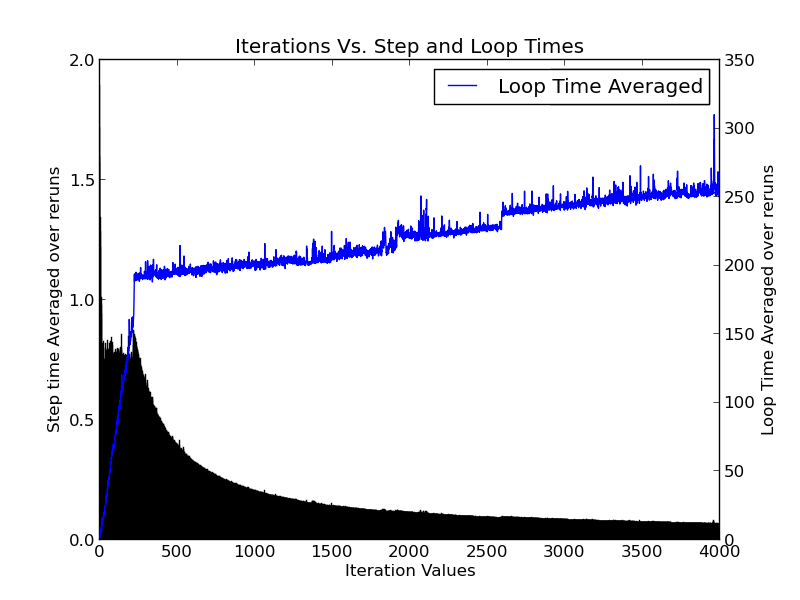
\includegraphics[scale=0.7]{./images/plot01.png}
\end{center}
\subsection{Observations from Plot 02}

There are five components of this graph. The averaged step time is similar in characteristics to that of first plot i.e. it decreases with increasing iteration values.

One another observation that can be made from this plot is that the line depicting average velocity time lies on the top i.e for all iteration values the average velocity time has the highest value as compared to collision and position times. And average position time is greater than collision time for all iteration values. Step time is actually the time taken to execute one iteration of the for loop so it is the sum of all velocity, position and collsion times plus something extra, thus step time is on the top. The variation in step time can be highly non-uniform owing to the fact that the collisions happening at some particular time can be very different in number from those happening at some other time. So it might happen that it peaks somewhere in the middle all of a sudden.
\begin{center}
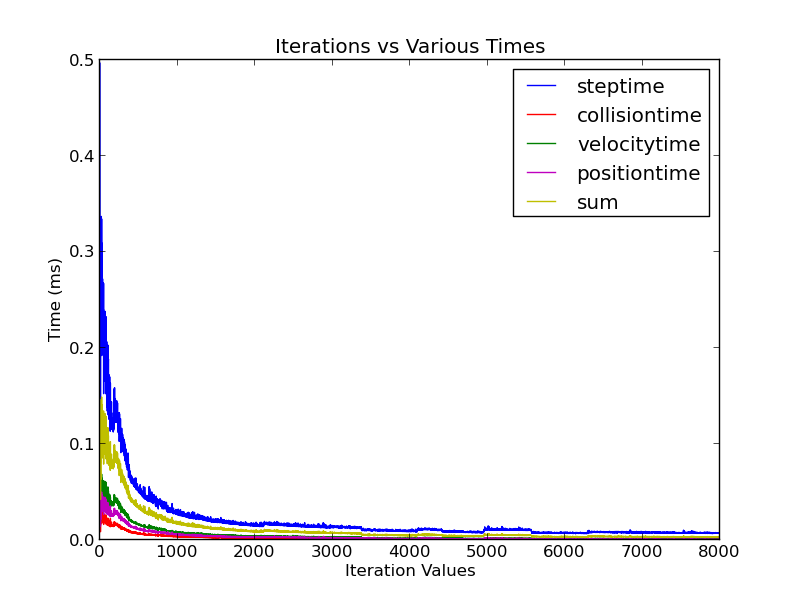
\includegraphics[scale=0.7]{./images/plot02.png}
\end{center}

\subsection{Observations from Plot 03}
In this plot the errors i.e. the variation in step times over reruns have been plotted alongwith the step time itself as line graph. A prominent observation which can be made is that error is very large initially and it gradually decreases as the iteration number increases. That is, for large iteration value the variation in step time is less.
 

\begin{center}
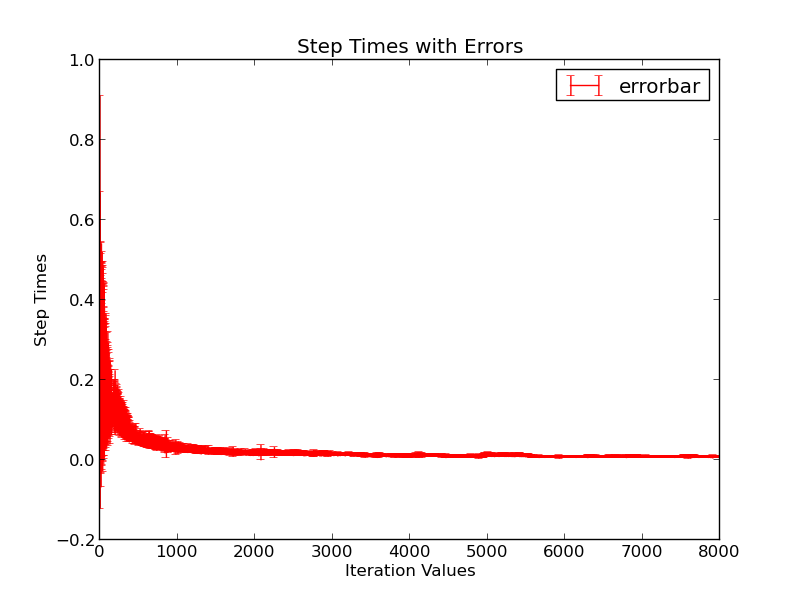
\includegraphics [scale=0.7]{./images/plot03.png}
\end{center}


\section{Profiling the code : An Investigation}
perf has been used to profile the code.\\
~\cite{perftut}.
~\cite{gp2dot}.
\begin{lstlisting}
perf record ./mybins/cs296_24_exe auto 20000 > /dev/null
perf script | python gprof2dot.py | dot -Tpng -o debug.png
\end{lstlisting}
The above code has been used to generate the necessary data and call graph images. 
\subsection{Debug and Release Modes}
Debug and Release are different configurations for building the project. Debug mode is used for debugging the project and the Release mode is used for the final build for users. Optimizations complicate the debugging process so the debug mode does not include optimizations and in addition it also generates some extra debug data. The Release mode enables optimizations and generates less debug data.\\

The above fact can be observed easily while running the code in both the modes. In release mode the code takes less time to run than in debug mode. For 20000 iterations the code when run in release mode took around 750ms and when run in debug mode the same code took around 6000ms to run.\\

Some optimizations reduce the size of the resulting machine code, while others try to create code that is faster, potentially increasing its size.
The optimization used in the base code is third level optimization i.e. -O3. In this level of optimization more emphasis is given on speed than size.

\subsection{Base code in Release Mode}
To compile the base code in release mode a small modification needs to be made. In place of 'cmake ../' , 'cmake -DCMAKE\_BUILD\_TYPE=Release ../' is used. The -On flag is included while compiling the base code.
The following output was observed when the code was run in release mode:\\
\begin{center}
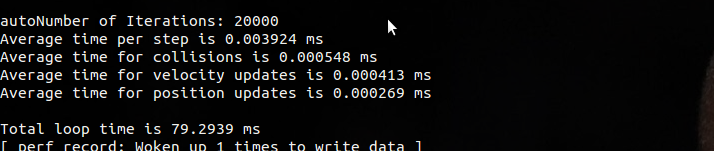
\includegraphics[scale=0.6]{./images/release.png}
\end{center}

\subsection{Base Code in Debug Mode}
To compile the base code in release mode a small modification needs to be made. In place of 'cmake ../' , 'cmake -DCMAKE\_BUILD\_TYPE=Debug ../' is used. The -On flag is removed while compiling the base code.
The following output was observed when the code was run in debug mode:\\
\begin{center}
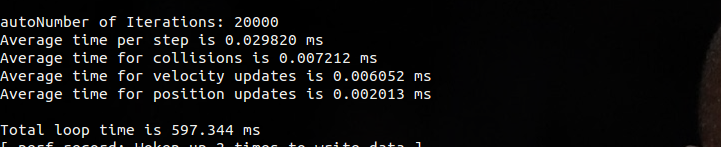
\includegraphics[scale=0.6]{./images/debug.png}
\end{center}



\section{Call Graph Images}
\subsection{Release Mode}
\begin{center}
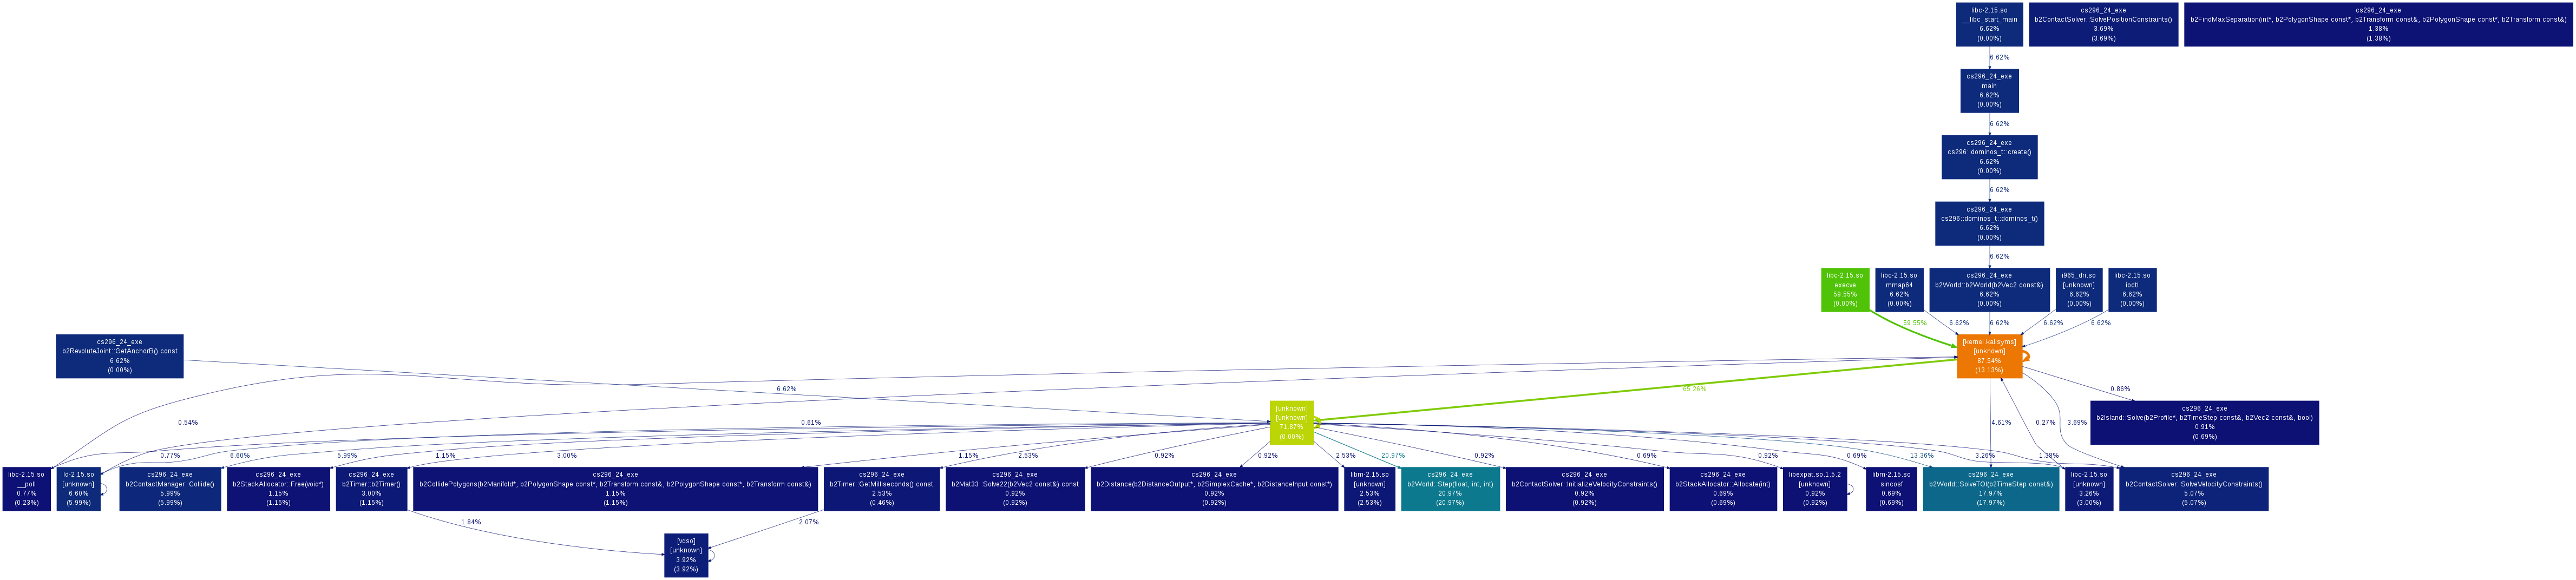
\includegraphics [scale=0.10]{./images/release_output.png}
\end{center}

\subsection{Debug Mode}
\begin{center}
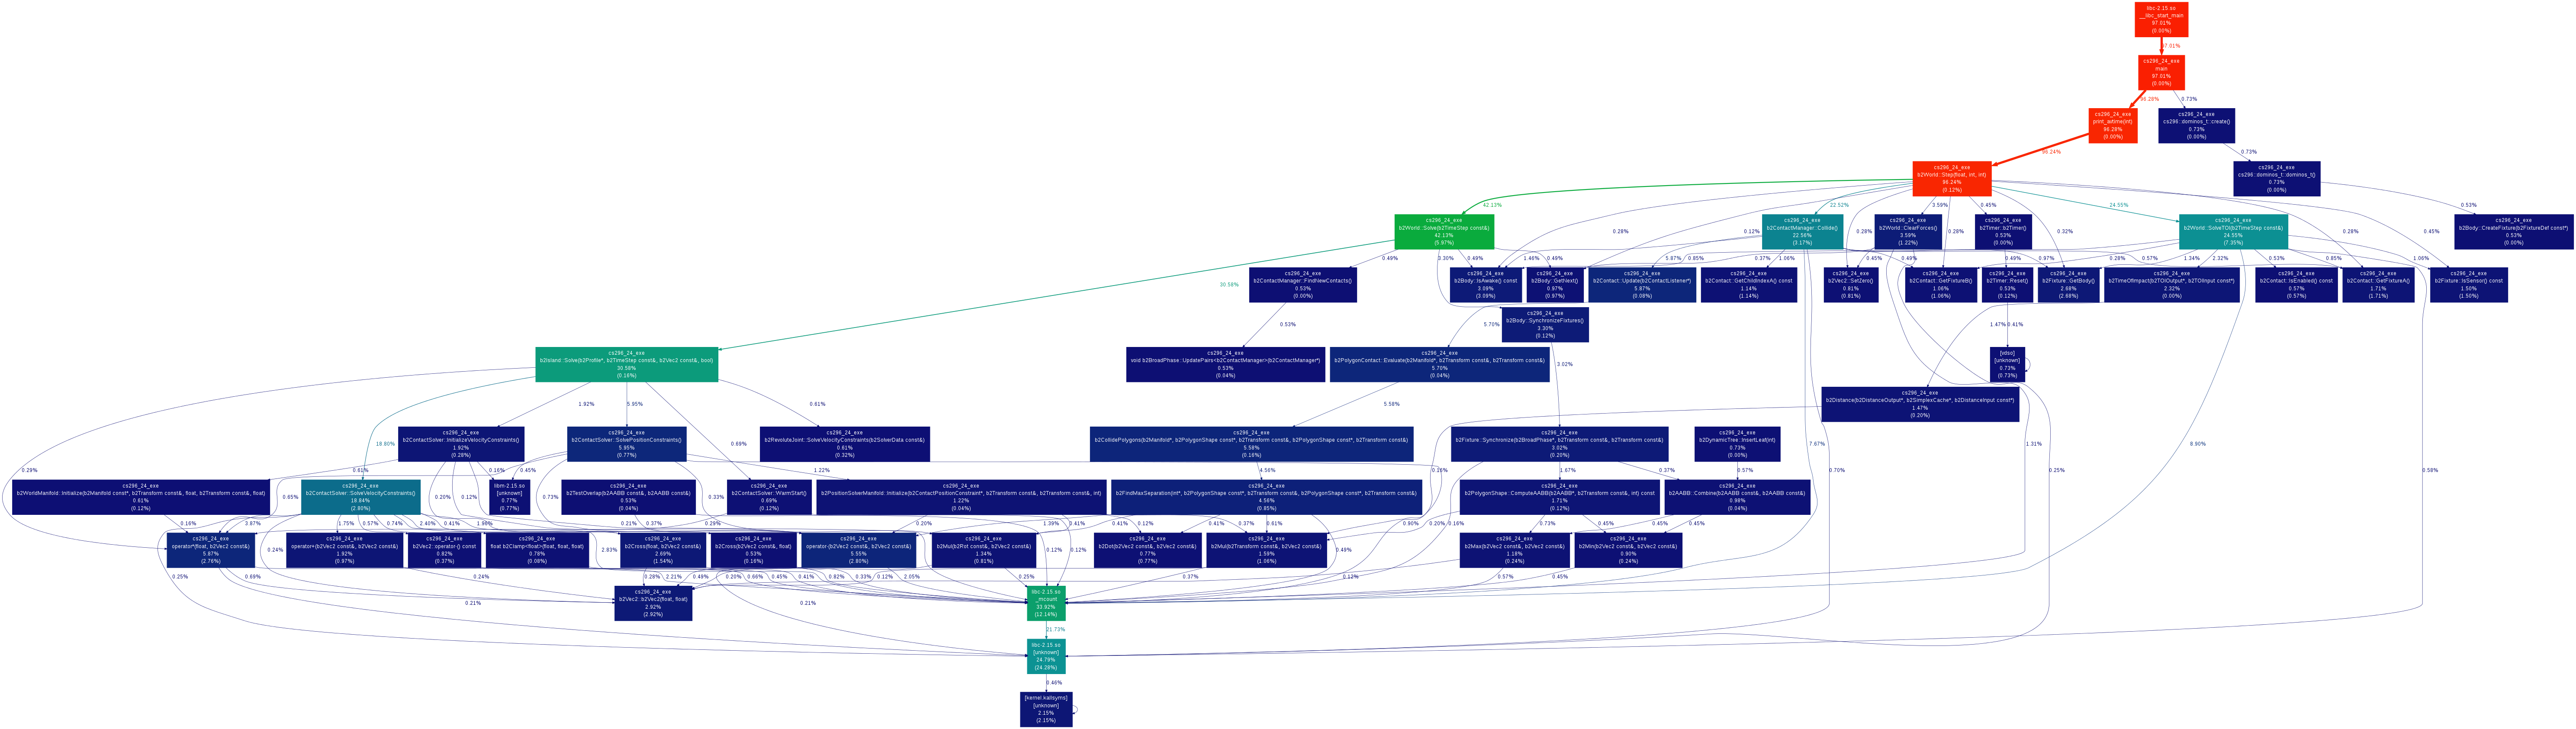
\includegraphics [scale=0.079]{./images/debug_output.png}
\end{center}

\section{Inferences drawn from the Call Graph}

1. The code has been run for 20000 iterations .\\ \\
2. In release mode, maximum time is taken by the function b2ContactSolver::SolveVelocityConstraints() which is 36.00\% whereas in debug mode, maximum time is taken by the same function\\ b2ContactSolver::SolveVelocityConstraints() but only 22.32\% .\\ \\
3. In release mode the function b2ContactListener::PostSolve(b2Contact*, b2ContactImpulse const*) has been called most number of times which is 394885 whereas in debug mode it is b2Vec2::b2Vec2(float, float) which has been called 111737403 times..\\ \\

\section{Required Optimizations}
Using the -O3 flag optimizes the code to make it run faster. It also turns on the inline-functions and rename-registers options. So we need to look at the functions which are not optimized even after using the -O3 options.\\

Therefore, the functions which are not being able to optimized in the release mode needs to be optimized. That is the functions whose \% time consumed does not change much from debug mode and release mode. We can safely assume that b2ContactSolver::SolveVelocityConstraints() function needs to be optimized.

\section{Conclusion}
After doing this assignment a lot of previously unknown things became clear.
The difference between release and debug modes, timing and profiling the code are some of the things which we came to know about after doing this assignment.
\bibliography{citation}
\end{document}

